\documentclass[12pt, titlepage]{article}

\usepackage{float}
\usepackage{booktabs}
\usepackage{longtable}
\usepackage{pdflscape}
\usepackage{tabularx}
\usepackage{hyperref}

\usepackage{fullpage}
\usepackage{multirow}
\usepackage{graphicx}
\usepackage{ulem}
\hypersetup{
    colorlinks,
    citecolor=black,
    filecolor=black,
    linkcolor=red,
    urlcolor=blue
}
\usepackage[round]{natbib}

\input{../Comments}
\input{../Common.tex}

\newcounter{acnum}
\newcommand{\actheacnum}{AC\theacnum}
\newcommand{\acref}[1]{AC\ref{#1}}

\newcounter{ucnum}
\newcommand{\uctheucnum}{UC\theucnum}
\newcommand{\uref}[1]{UC\ref{#1}}

\newcounter{mnum}
\newcommand{\mthemnum}{M\themnum}
\newcommand{\mref}[1]{M\ref{#1}}

\begin{document}

\title{Verification and Validation Report: \progname} 
\author{\authname}
\date{\today}
	
\maketitle

\pagenumbering{roman}

\section{Revision History}

\begin{tabularx}{\textwidth}{p{3cm}p{2cm}X}
\toprule {\bf Date} & {\bf Version} & {\bf Notes}\\
\midrule
2025-03-10 & 1.0 & Initial Report\\

\bottomrule
\end{tabularx}

~\newpage

\section{Symbols, Abbreviations and Acronyms}

\renewcommand{\arraystretch}{1.2}
\begin{tabular}{l l} 
  \toprule		
  \textbf{symbol} & \textbf{description}\\
  \midrule 
  T & Test\\
  SRS & Software Requirements Specification\\
  MG & Module Guide\\
  MIS & Module Interface Specification\\
  FR & Functional Requirements\\
  NFR & Non-Functional Requirements\\
  UI & User Interface\\
  MFA & Multi-Factor Authentication \\
  MG & Module Guide \\
  M & Module \\
  MIS & Module Interface Specification \\
  API & Application Programming Interface \\
  MFA & Multi-Factor Authentication \\
  IR & Integrity Requirement\\
  AR & Access Requirement\\
  \bottomrule
\end{tabular}\\

% \wss{symbols, abbreviations or acronyms -- you can reference the SRS tables if needed}

\newpage

\tableofcontents

\listoftables 

\listoffigures

\newpage

\pagenumbering{arabic}

This document summarizes the results of series of tests as outlined in the VnV Plan, demonstrating the system's compliance with the specified requirements and highlighting areas of success as well as any identified issues. \\

\section{Functional Requirements Evaluation} \label{section:3} 

\subsection{Add a document to the database} \label{section:3.1}

This subsection covers FR1, FR4, and FR8 from of the \href{https://github.com/Inreet-Kaur/capstone/blob/main/docs/SRS/SRS.pdf}{SRS document} by testing that the system is able to add a document to the database only when a valid input is provided.

\begin{enumerate}

  \item{test-FR1,4,8-1} \label{test-FR1,4,8-1}
  
  Initial State: The system is set up, open to the relevant section (e.g., Healthcare Network, Healthcare Professional, or Patient Records), and ready to take the user input.

  Input: Correct and complete input data for all required fields.

  Expected Output: A confirmation message and a new entry is added to the appropriate database.

  Actual Output: A confirmation message and a new entry is added to the appropriate database.

  Result: Pass


  \item{test-FR1,4,8-2} \label{test-FR1,4,8-2}

  Initial State: The system is set up, open to the relevant section (e.g., Healthcare Network, Healthcare Professional, or Patient Records), and ready to take the user input.

  Input: Invalid input data.

  Expected Output: An error message outlining the invalid fields along with a possible steps to guide the users to recover from the error state.

  Actual Output: An error message outlining the invalid fields along with a possible steps to guide the users to recover from the error state.

  Result: Pass

\end{enumerate}

\subsection{Remove a document to the database} \label{section:3.2}

This subsection covers FR2, FR5, and FR9 from of the \href{https://github.com/Inreet-Kaur/capstone/blob/main/docs/SRS/SRS.pdf}{SRS document} by testing that the system is able to remove a document to the database only when a valid input idetifier is provided.

\begin{enumerate}

  \item{test-FR2,5,9-1} \label{test-FR2,5,9-1}
  
  Initial State: The system is set up, open to the relevant section (e.g., Healthcare Network, Healthcare Professional, or Patient Records), and ready to take the user input. A document exists in the appropriate database.

  Input: A correct identifier for the document to be deleted.

  Expected Output: A confirmation message and relevant entry no longer exist in the database.

  Actual Output: A confirmation message and relevant entry no longer exist in the database.

  Result: Pass


  \item{test-FR2,5,9-2} \label{test-FR2,5,9-2}

  Initial State: The system is set up, open to the relevant section (e.g., Healthcare Network, Healthcare Professional, or Patient Records), and ready to take the user input. A document exists in the appropriate database.

  Input: An invalid identifier for the document to be deleted.

  Expected Output: An error message outlining the invalid input along with a possible steps to guide the users to recover from the error state.

  Actual Output: An error message outlining the invalid input along with a possible steps to guide the users to recover from the error state.

  Result: Pass

\end{enumerate}

\subsection{Update a document to the database} \label{section:3.3}

This subsection covers FR3, FR6, FR10, and FR11 from of the \href{https://github.com/Inreet-Kaur/capstone/blob/main/docs/SRS/SRS.pdf}{SRS document} by testing that the system is able to update a document to the database only when a valid input idetifier is provided.

\begin{enumerate}

  \item{test-FR3,6,10,11-1} \label{test-FR3,6,10,11-1}
  
  Initial State: The system is set up, open to the relevant section (e.g., Healthcare Network, Healthcare Professional, or Patient Records), and ready to take the user input.

  Input: A correct identifier for the document to be updated.

  Expected Output: A confirmation message and relevant entry shows the updated data in the database.

  Actual Output: A confirmation message and relevant entry shows the updated data in the database.

  Result: Pass


  \item{test-FR3,6,10,11-2} \label{test-FR3,6,10,11-2}

  Initial State:  The system is set up, open to the relevant section (e.g., Healthcare Network, Healthcare Professional, or Patient Records), and ready to take the user input.

  Input: Invalid input data.

  Expected Output: An error message outlining the invalid fields along with a possible steps to guide the users to recover from the error state.

  Actual Output: An error message outlining the invalid fields along with a possible steps to guide the users to recover from the error state.

  Result: Pass

\end{enumerate}

\subsection{Login for valid/invalid credentials} \label{section:3.4}

This subsection covers FR7 from of the \href{https://github.com/Inreet-Kaur/capstone/blob/main/docs/SRS/SRS.pdf} {SRS document} by testing that the system is able to allow to access the database only when a valid input credentials is provided.

\begin{enumerate}

  \item{test-FR7-1} \label{test-FR7-1}
  
  Initial State:  The system is set up, and the user is on the login page, ready to enter their credentials.

  Input: The correct credentials for login.

  Expected Output: A confirmation message and user is logged into the system.

  Actual Output: A confirmation message and user is logged into the system.

  Result: Pass


  \item{test-FR7-2} \label{test-FR7-2}

  Initial State:  The system is set up, and the user is on the login page, ready to enter their credentials.

  Input: Invalid credentials for login.

  Expected Output: An error message outlining the invalid fields.

  Actual Output: An error message outlining the invalid fields.

  Result: Pass

\end{enumerate}

\subsection{Voice-to-text-transcription check} \label{section:3.5}

This subsection covers FR7 from of the \href{https://github.com/Inreet-Kaur/capstone/blob/main/docs/SRS/SRS.pdf} {SRS document} by testing that the system is able to transcribe audio data to the written text.

\begin{enumerate}

  \item{test-FR11-1} \label{test-FR11-1}
  
  Initial State: The user has successfully logged in and is on the appropriate view to take audio input. 

  Input: A valid audio chunk from the conversation between the healthcare professional and the patient.

  Expected Output: A confirmation message indicating successful transcription and the screen shows the transcribed text.

  Actual Output: A confirmation message indicating successful transcription and the screen shows the transcribed text.

  Result: Pass


  \item{test-FR11-2} \label{test-FR11-2}

  Initial State: The user has successfully logged in and is on the appropriate view to take audio input.

  Input: An invalid data format for transcription.

  Expected Output: An error message saying that the file or data format is not valid.

  Actual Output: An error message saying that the file or data format is not valid.

  Result: Pass

\end{enumerate}

\subsection{Validate output of correct diagnosis and medication} \label{section:3.6}

This subsection covers FR12 and FR13 from of the \href{https://github.com/Inreet-Kaur/capstone/blob/main/docs/SRS/SRS.pdf} {SRS document} by testing that the system is able to create predictions on the diagnosis and medicines with a high accuracy and confidence.

\begin{enumerate}

  \item{test-FR12,13-1} \label{test-FR12,13-1}
  
  Initial State: Patient's blank chart is present, and a transcription of the Patient-Healthcare Professional conversation is present.

  Input: Correct and complete input data where all the symptoms fields of the chart are filled out.

  Expected Output: A suggestion on what the diagnosis should be based on the symptoms, then based on the diagnosis provide possible medicine and a plan of treatment.

  Actual Output: A suggestion on what the diagnosis should be based on the symptoms, then based on the diagnosis provide possible medicine and a plan of treatment.

  Result: Pass

\end{enumerate}


\subsection{Validate input data for models} \label{section:3.7}

This subsection covers FR12, FR13, and IR5 from of the \href{https://github.com/Inreet-Kaur/capstone/blob/main/docs/SRS/SRS.pdf} {SRS document} by testing that the system is able to validate the input data in the charts such that it may be inputted into the prediction module.

\begin{enumerate}

  \item{test-FR12,13,IR5-1} \label{test-FR12,13,IR5-1}
  
  Initial State: The patient's blank chart is present.

  Input: Correct and complete input data where the transcription is present.

  Expected Output: A suggestion on what the diagnosis should be based on the symptoms, then based on the diagnosis provide possible medicine.

  Actual Output: A suggestion on what the diagnosis should be based on the symptoms, then based on the diagnosis provide possible medicine.

  Result: Pass

  \item{test-FR12,13,IR5-2} \label{test-FR12,13,IR5-2}
  
  Initial State: The patient's blank chart is present.

  Input: Incorrect and incomplete transcription field as it was not recorded/complete.

  Expected Output: An error message relaying the error along with a HTTP status code indicating incomplete request.

  Actual Output: An error message relaying the error along with a HTTP status code indicating incomplete request.

  Result: Pass

\end{enumerate}

\section{Nonfunctional Requirements Evaluation} \label{section:4}

\subsection{Aesthetic and Design} \label{section:4.1}

\begin{enumerate}

  \item {test-AD1} \label{test-AD1}

  Initial State: UI is designed and implemented.

  Input: Team members and peers view the UI under normal operating conditions.

  Output: Feedback collected on UI’s aesthetic appeal and simplicity.

  Result: Pass

  \item {test-AD2} \label{test-AD2}

  Initial State: UI is operational and accessible to users.

  Input: Users interact with the UI during routine tasks and provide feedback.

  Output: Team members and peers report satisfaction with the UI design.

  Result: Pass

\end{enumerate}

\subsection{Usability} \label{section:4.2}

\begin{enumerate}

  \item {test-UR1} \label{test-UR1}

  Initial State: System is deployed and accessible.

  Input: Users navigate and explore system features independently.

  Output: Majority of users can locate core functions without additional guidance.

  Result: Pass

\end{enumerate}

\subsection{Performance} \label{section:4.3}

\begin{enumerate}
\item test-PR1 \label{test-PR1}

Initial State: Transcription interface open and ready.

Input: Real-time voice input provided by healthcare professionals.

Output: Real-time transcription displayed within a 2-second delay.

Result: Pass 

\end{enumerate}

\subsection{Operational} \label{section:4.4}

\begin{enumerate}
\item test-OR1 \label{test-OR1}

Initial State: System is running in a controlled test environment.

Input: Multiple test users perform basic interactions (e.g., logging in, recording voice input, retrieving stored data).

Output: The system responds within an acceptable time frame, and no critical errors occur.

Result: Pass

\end{enumerate}

\subsection{Maintainability} \label{section:4.5}

\begin{enumerate}
  \item test-MR1 \label{test-MR1}
  
  Initial State: System is running in the development environment.
  
  Input: Review and modify system components (e.g., refactoring code, adding new functionality).
  
  Output: Changes are successfully integrated without breaking existing functionality, verified through automated/unit tests.
  
  Result: Pass

  \item test-MR2 \label{test-MR2} 

  Initial State: Codebase is under active development.
  
  Input: Perform a code maintainability review i.e. checking adherence to coding standards, documentation completeness.
  
  Output: Code follows maintainability best practices, including clear documentation and modular structure.
  
  Result: Pass/Fail
  \end{enumerate}

\end{enumerate}

\subsection{Security} \label{section:4.6}

\begin{enumerate}
\item test-SR1 \label{test-SR1}

Initial State: System fully operational with access logs enabled.

Input: Simulate unauthorized access attempts.

Output: Unauthorized attempts are blocked; access logs capture details.

Result: Pass

\end{enumerate}

\subsection{Cultural} \label{section:4.7}

\begin{enumerate}
\item test-CR1 \label{test-CR1} 

Initial State: System operational with default settings.

Input: User interacts with the system in a culturally diverse context, including input that may contain sensitive language.

Output: System processes the input and responds appropriately, ensuring cultural sensitivity and avoiding any inappropriate language in its output.

Result: Pass

\end{enumerate}

\subsection{Legal} \label{section:4.8}

\begin{enumerate}
\item test-LR1 \label{test-LR1}

Initial State: System is fully functional and contains patient records.

Input: Conduct a compliance audit with PIPEDA and other relevant data protection standards.

Output: System passes all compliance checks with no exceptions.

Result: Pass

\item test-LR2 \label{test-LR2}

Initial State: System storing and transmitting patient data over a network.

Input: Monitor data handling and transfer processes during operation.

Output: All patient data is handled in compliance with regulations, without any unauthorized access or data breaches.

Result: Pass

\end{enumerate}

\subsection{Scalability} \label{section:4.9}

\begin{enumerate}
\item test-S1 \label{test-S1}

Initial State: System deployed on a test server environment capable of scaling horizontally.

Input: Simulate an increasing number of concurrent users.

Output: System maintains consistent performance and response times without degradation.

Result: Pass

\end{enumerate}

\subsection{Tests for Safety and Security Requirements} \label{section:4.10}

\subsubsection{Access Requirements Tests (AC1)} \label{section:4.10.1}

\begin{enumerate}
\item test-AC1-1 \label{test-AC1-1}

Initial State: System deployed with authentication module enabled and test user accounts configured.

Input: Attempt to access protected resources with invalid credentials.

Output:
\begin{itemize}
\item System logs each failed attempt.
\item User receives failed to login notification.
\end{itemize}

Result: Pass

\item test-AC1-2 \label{test-AC1-2}

Initial State: System operational with authentication logs enabled.

Input: Attempt to access system resources without authentication.

Output: 
\begin{itemize}
    \item All unauthorized access attempts are blocked.
    \item Each attempt is logged with timestamp, IP address, and attempted resource.
\end{itemize}

Result: Pass

\item test-AC2-1 \label{test-AC2-1}

Initial State: System operational with standard user and admin accounts configured.

Input: Attempt to create, update, and delete user accounts using non-admin credentials.

Output:
\begin{itemize}
\item All unauthorized actions are blocked.
\item Actions are logged with user details.
\item Security team can review blocked attempts.
\end{itemize}

Result: Pass

\end{enumerate}

\subsubsection{Integrity Requirements Tests (IR1)} \label{section:4.10.2}

\begin{enumerate}

  \item test-IR1-1 \label{test-IR1-1}

  Initial State: System operational with test user accounts and authentication database.

  Input: Simulate multiple concurrent failed login attempts while monitoring credential storage.


  Output: User credentials remain unchanged, and system maintains stability.

  Result: Pass

  \item test-IR2-1 \label{test-IR2-1}

  Initial State: System is set up, open to the relevant section, and ready to take user input.

  Input: Submit an invalid data input.

  Output: An error message is displayed to the user. No data is added to any database.

  Result: Pass

  \item test-IR3-1 \label{test-IR3-1}

  Initial State: The prediction model is ready to predict medication and diagnosis.

  Input: A test set of various patient medical charts.

  Output: The prediction includes a diagnosis and medication prediction, each with a confidence score exceeding 85\%.

  Result: Pass

  \item test-IR4-1 \label{test-IR4-1}

  Initial State: System is set up, open to the relevant section, and ready to take user input. A document already exists in the relevant database.

  Input: A new input with the same data as an existing document.

  Output: An error message is displayed. No new document is added to the database.

  Result: Pass

  \item test-IR5-1 \label{test-IR6-1} 
  
  Initial State: System is set up, open to the relevant section, and ready to take user input. A document already exists in the relevant database.

  Input: Written text transcribed from the audio data.

  Output: The data is correctly classified in the generated report with no diagnosis errors.

  Result: Pass

  \item test-IR6-1 \label{test-IR7-1}

  Initial State: System is set up, open to the relevant section, and ready to take user input.

  Input: Audio conversation between the patient and healthcare professional.

  Output: The written text transcribed from the input data matches the conversation with minimal to no interference.

  Result: Pass

\end{enumerate}


\section{Comparison to Existing Implementation}	

N/A

\section{Unit Testing}

\subsection{Behaviour-Hiding Module}

\subsubsection{User Authentication Module}

  \textbf{Control:} Manual \\
  \textbf{Initial State:} The default email and password are initialized as variables and given a default value.\\
  \textbf{Test Case Derivation:} The expected behavior is derived from the correct registration and login functionality of Firebase Authentication, ensuring valid user creation and authentication processes, as well as error handling for invalid credentials.\\
  \textbf{Test Procedure:} The tests are performed as follows:
  \begin{enumerate}
    \item Sign up using valid credentials:
      \begin{itemize}
        \item \textbf{Input:} The input for this test are the valid credentials of email and password.
        \item \textbf{Output:} The user object is returned by the signup function.
        \item \textbf{Test Derivation:} Verifies that the signup function correctly works and creates a new user account when the valid credentials are provided.
        \item \textbf{Result:} Pass 
      \end{itemize}

    \item Sign up throwing errors with invalid credentials:
      \begin{itemize}
        \item \textbf{Input:} The input for this test are the invalid credentials of email and password.
        \item \textbf{Output:} An error thrown up by the signup function.
        \item \textbf{Test Derivation:} Verifies that the signup function correctly throws error when the invalid credentials are provided.
        \item \textbf{Result:} Pass 
      \end{itemize}

    \item Sign in using valid credentials:
      \begin{itemize}
        \item \textbf{Input:} The input for this test are the valid credentials of email and password. 
        \item \textbf{Output:} The user object is returned by the signin function.
        \item \textbf{Test Derivation:}  Verifies that the signin function correctly authenticates the user when valid credentials are provided.
        \item \textbf{Result:} Pass 
      \end{itemize}

    \item Sign in throwing errors with invalid credentials:
      \begin{itemize}
        \item \textbf{Input:} The input for this test are the invalid credentials of email and password. 
        \item \textbf{Output:} An error thrown up by the signin function.
        \item \textbf{Test Derivation:} Verifies that the signin function correctly throws error when the invalid credentials are provided.
        \item \textbf{Result:} Pass 
      \end{itemize}
  \end{enumerate}


\subsubsection{Administrator Account Management Module and Patient Account Management Module}

  \textbf{Control:} Manual\\
  \textbf{Initial State:} Provides mock data of healthcare professionals, healthcare networks and patients.\\
  \textbf{Test Case Derivation:} The expected behavior is derived from the correct functionality of onboarding, updating, and removing the healthcare networks, healthcare professionals and patient records.\\
  \textbf{Test Procedure:} The tests are performed as follows:
  \begin{enumerate}
    \item Adding valid documents to the database:
      \begin{itemize}
        \item \textbf{Input:} Mock data of the healthcare professionals, healthcare networks and patients are given as input.  
        \item \textbf{Output:} Successful addition of valid information of healthcare networks, healthcare professionals and patients in the database. 
        \item \textbf{Test Derivation:} Verifies that addHealthcareProfessional, addHospital and addPatient functions work correctly ensuring proper document creation. The functions addHealthcareProfessional and addHospital add the documents if they don't exist in the database. However, if they do, then these functions update the data in those documents. The function addPatient is only used to add a new patient record in the database.
        \item \textbf{Result:} Pass 
      \end{itemize}

    \item No duplicate addition of patient document in the system:
      \begin{itemize}
        \item \textbf{Input:} Mock data of the patients are given as input.  
        \item \textbf{Output:} No specific output is returned by the test function itself. However, the test asserts a specific state in the database. 
        \item \textbf{Test Derivation:} Verifies that the addPatient function correctly handles attempts to add duplicate patient records. It ensures that only one patient record is created even if the addPatient function is called multiple times.
        \item \textbf{Result:} Pass
      \end{itemize}

      Note: Test for invalid document format: \\
      Since, we have implemented validate input function in the UI module, this ensures that no invalid output is taken by the system. In addition to this, TypeScript has type checking on the parameters therefore invalid objects cannot be passed.

    \item Deleting existing documents from the database:
      \begin{itemize}
        \item \textbf{Input:} Mock data of the healthcare professionals, healthcare networks and patients are given as input.  
        \item \textbf{Output:} Successful deletion of valid information of healthcare networks, healthcare professionals and patients in the database. 
        \item \textbf{Test Derivation:} Verifies that deleteHealthCareProfessional, deleteHospital and deletePatient functions work correctly ensuring proper document deletion.
        item \textbf{Result:} Pass
      \end{itemize}

    \item Updating existing patient documents in the database:
      \begin{itemize}
        \item \textbf{Input:} Mock data of the patients are given as input.  
        \item \textbf{Output:} Successful update of valid information of the patients in the database. 
        \item \textbf{Test Derivation:} Verifies that updatePatient function works correctly ensuring proper patient record update.
        \item \textbf{Result:} Pass
      \end{itemize}

    \item Retrieve correct existing document:
      \begin{itemize}
        \item \textbf{Input:} Mock id of the patients are given as input.  
        \item \textbf{Output:} Retrieval of the correct patient object from the database. 
        \item \textbf{Test Derivation:} Verifies that the getPatient function correctly retrieves an existing patient document from the database after providing patient id.
        \item \textbf{Result:} Pass
      \end{itemize}

    \item Retrieve non-existing document:
      \begin{itemize}
        \item \textbf{Input:} Non-existent mock id of the patients are given as input.  
        \item \textbf{Output:} Returns null. 
        \item \textbf{Test Derivation:} Verifies that the getPatient function correctly handles situations when a non-existing patient document from the database is requested to retrieve after providing a non-existing patient id.
        \item \textbf{Result:} Pass
      \end{itemize}
  \end{enumerate}

\subsubsection{Administrator View Module and Patient View Module}

  \textbf{Control:} Manual\\
  \textbf{Initial State:} No specific initialization is required as tests solely focus on validating fields.\\
  \textbf{Test Case Derivation:} The expected behavior is derived from the correct implementation of data validation rules and age calculation logic, ensuring accurate identification of invalid input, acceptance of valid input, and precise calculation of age based on provided dates.\\
  \textbf{Test Procedure:} The tests are performed as follows:\\

  \begin{enumerate}
    \item Should return appropriate error for invalid field input:
      \begin{itemize}
        \item \textbf{Input:} The inputs for this test are the actual value of the field and a string representing the field type.   
        \item \textbf{Output:} Returns appropriate error messages on receiving invalid input.
        \item \textbf{Test Derivation:} Verifies that the validateField function correctly identifies invalid input values for different field types. It ensures that the function returns appropriate error messages for invalid email formats, phone numbers, dates, and numerical values for age, weight, and height.
        \item \textbf{Result:} Pass
      \end{itemize}

    \item Should return an empty string for valid field input:
      \begin{itemize}
        \item \textbf{Input:} The inputs for this test are the actual value of the field and a string representing the field type.   
        \item \textbf{Output:} Returns an empty string on receiving invalid input.
        \item \textbf{Test Derivation:} Verifies that the validateField function correctly identifies valid input values for different field types. It ensures that the function returns an empty string for valid email formats, phone numbers, dates, and numerical values for age, weight, and height.
        \item \textbf{Result:} Pass
      \end{itemize}

    \item Correct calculation of age:
      \begin{itemize}
        \item \textbf{Input:} The input for this test is the date of birth.    
        \item \textbf{Output:} Returns a number representing the calculated age.
        \item \textbf{Test Derivation:} Verifies that the calculateAge function correctly calculates the age for a given date of birth.
        \item \textbf{Result:} Pass
      \end{itemize}

    \item Calculation of age for future dates:
      \begin{itemize}
        \item \textbf{Input:} The input for this test is the date of birth in the future.    
        \item \textbf{Output:} Returns 0.
        \item \textbf{Test Derivation:} Verifies that the calculateAge function correctly handles the age for a given date of birth in the future.
        \item \textbf{Result:} Pass
      \end{itemize}

    \item Calculation of age for the present date:
      \begin{itemize}
        \item \textbf{Input:} The input for this test is the date of birth representing today's date.    
        \item \textbf{Output:} Returns 0.
        \item \textbf{Test Derivation:} Verifies that the calculateAge function correctly handles the age for a given date of birth with today's date.
        \item \textbf{Result:} Pass
      \end{itemize}
  \end{enumerate}

  \subsection{Software Decision Module}

  \subsubsection{Diagnosis Prediction Module and Medicine Prediction Module}

  \textbf{Control:} Automatic\\
  \textbf{Initial State:} A predefined set of conversation is used for testing. It also assumes that Open API Key is configured correctly.\\
  \textbf{Test Case Derivation:} The expected behavior is derived from the correct functioning of an API endpoint that processes patient inputs and provides relevant responses, ensuring accurate handling of valid and invalid input data, as well as a high confidence level in generating appropriate responses. We will review the manual test by our supervisor.
  \textbf{Test Procedure:} The tests are performed as follows:\\

  \begin{enumerate}
    \item Confidence score test:
      \begin{itemize}
        \item \textbf{Input:} The input for this test is the list of strings which represent patient conversation.   
        \item \textbf{Output:} There is no direct output. This test asserts a condition based on the number of successful evaluations.
        \item \textbf{Test Derivation:} Verifies that the testConfidence function correctly sends each conversation to the API endpoint. The test calculates the success rate based on the number of relevant responses and asserts that the success rate is above a certain threshold (0.85). Due to the output of this test not being the deterministic, we have used a strategy that involves using a third independent AI agent to evaluate the confidence. This allows for an initial benchmark of the confidence on the service's performance. 
        \item \textbf{Result:} Pass
      \end{itemize}

    \item Valid data input test:
      \begin{itemize}
        \item \textbf{Input:} A dictionary that contains a valid transcription of a patient conversation. 
        \item \textbf{Output:} Returns a response object from API endpoint.
        \item \textbf{Test Derivation:} Verifies that the API endpoint correctly handles and processes valid input data. It sends POST request with valid transcription to the API endpoint and asserts that the response status code is 200, indicating successful processing of the input.
        \item \textbf{Result:} Pass
      \end{itemize}

    \item Invalid data input test:
      \begin{itemize}
        \item \textbf{Input:} A dictionary that contains an empty string of invalid transcription of a patient conversation.    
        \item \textbf{Output:} Returns a response object from API endpoint.
        \item \textbf{Test Derivation:} Verifies that the API endpoint correctly handles and processes invalid input data. It sends POST request with invalid and missing transcription to the API endpoint and asserts that the response status code is 400, successful identification of invalid input.
        \item \textbf{Result:} Pass
      \end{itemize}
  \end{enumerate}

  \subsubsection{Transcription Module}

  \textbf{Control:} Manual\\
  \textbf{Initial State:} The audio files are provided as input for the tests and Socket.IO Server is running at a specified host.\\
  \textbf{Test Case Derivation:} The expected behavior is derived from the correct functioning of a Socket.IO server that receives audio chunks, performs transcription, and emits transcription results or errors. The tests ensure that the server correctly transcribes valid audio data, handles invalid audio input, and emits appropriate events with accurate transcription results or error indicators.\\
  \textbf{Test Procedure:} The tests are performed as follows:\\

  \begin{enumerate}
    \item Test for valid audio file:
      \begin{itemize}
        \item \textbf{Input:} The input for this test is the path to the valid audio file.   
        \item \textbf{Output:} Returns a string containing transcribed text from the audio file.
        \item \textbf{Test Derivation:} Verifies the audio transcription functionality of the Socket.IO server. It establishes a connection with the server and sends the audio data in chunks and then emits the transcribed text. 
        \item \textbf{Result:} Pass
      \end{itemize}

    \item Test for invalid audio file:
      \begin{itemize}
        \item \textbf{Input:} The input for this test is the path to the invalid audio file. 
        \item \textbf{Output:} Returns an empty string containing transcribed text from the audio file.  
        \item \textbf{Test Derivation:} Verifies that the API endpoint correctly handles invalid input data. It establishes the connection with the server and asserts that transcription\_text remains empty indicating that the invalid input is correctly handled.
        \item \textbf{Result:} Pass
      \end{itemize}
  \end{enumerate}

  \subsubsection{Classification Module}

  \textbf{Control:} Automatic\\
  \textbf{Initial State:} A list of pre-defined conversation containing patient's symptoms, allergies, medications is initialized.\\
  \textbf{Test Case Derivation:} The expected behavior is derived from the correct functioning of an API endpoint that processes patient conversations, extracts key information (symptoms, reason for visit, allergies, current medications), and provides relevant responses. The tests ensure that the API accurately extracts information from various conversation formats, handles both valid and invalid input data, and maintains a high level of confidence in generating appropriate responses.\\
  \textbf{Test Procedure:} The tests are performed as follows:\\

  \begin{enumerate}
    \item Confidence score test:
      \begin{itemize}
        \item \textbf{Input:} The input for this test is the list of strings representing the patient conversation consisting of medications, allergies and current medications.   
        \item \textbf{Output:} There is no direct output. This test asserts a condition based on the number of successful evaluations.
        \item \textbf{Test Derivation:} Verifies the confidence of the API in correctly extracting information from patient conversations. It iterates through the list sending conversation to the API endpoint. We will test it manually with our supervisor. 
        \item \textbf{Result:} Pass
      \end{itemize}

    \item Test for valid input:
      \begin{itemize}
        \item \textbf{Input:} The input for this test is the valid patient transcription. 
        \item \textbf{Output:} Returns a response object from the API endpoint. 
        \item \textbf{Test Derivation:} Verifies that the API endpoint correctly handles and processes valid input data. It sends POST request with valid input to the API endpoint and asserts that the response status code is 200, indicating successful processing of the input.
        \item \textbf{Result:} Pass
      \end{itemize}

      \item Test for invalid input:
      \begin{itemize}
        \item \textbf{Input:} The input for this test is an empty dictionary. 
        \item \textbf{Output:} Returns a response object from the API endpoint. 
        \item \textbf{Test Derivation:} Verifies that the API endpoint correctly handles empty input data. It sends POST request with empty input to the API endpoint and asserts that the response status code is 400, indicating successful processing of the input.
        \item \textbf{Result:} Pass
      \end{itemize}
  \end{enumerate}


\section{Changes Due to Testing}

% \wss{This section should highlight how feedback from the users and from 
% the supervisor (when one exists) shaped the final product.  In particular 
% the feedback from the Rev 0 demo to the supervisor (or to potential users) 
% should be highlighted.}
Based on the feedback received during the Rev 0 demo, we focused on ensuring that we prioritize critical and necessary requirements in the final implementation. We incorporated user feedback messages in accordance with the functional tests. Additionally, we updated the functions responsible for validating input data to cover the edge cases discovered during testing, ensuring that the system can handle unexpected or invalid inputs gracefully. Furthermore, we placed a strong emphasis on UI and usability testing. This involved gathering feedback on the aesthetic appeal and functionality of the user interface, ensuring that users could navigate the system intuitively and efficiently. Iterative testing process allowed us to refine the system significantly and make several design adjustments leading to a more user-friendly application.

\section{Automated Testing}

We useD GitHub Actions to automate critical aspects of our development workflow, primarily focusing on testing and code quality. This automation ensures that every code change undergoes a rigorous validation process before being integrated into the main branch. The execution of suite of unit and integration tests forms the basis of our continuous integration approach. This makes sure that any new code modifications don't cause regressions or interfere with already-existing functionality. These tests are automatically executed on each pull request, allowing us to promptly detect and fix any possible problems early in the development cycle. Our team has been continuously running into linting problems on all pull requests lately. Even though our tests pass GitHub Actions CI / Explore-GitHub-Actions (push) test, it fails the Lint code base (push) test. The screenshot below show an example of lint-codebase error. We hope to resolve this issue before final demonstration by fixing all the lint errors in the code.

\begin{figure}[h]
  \centering
  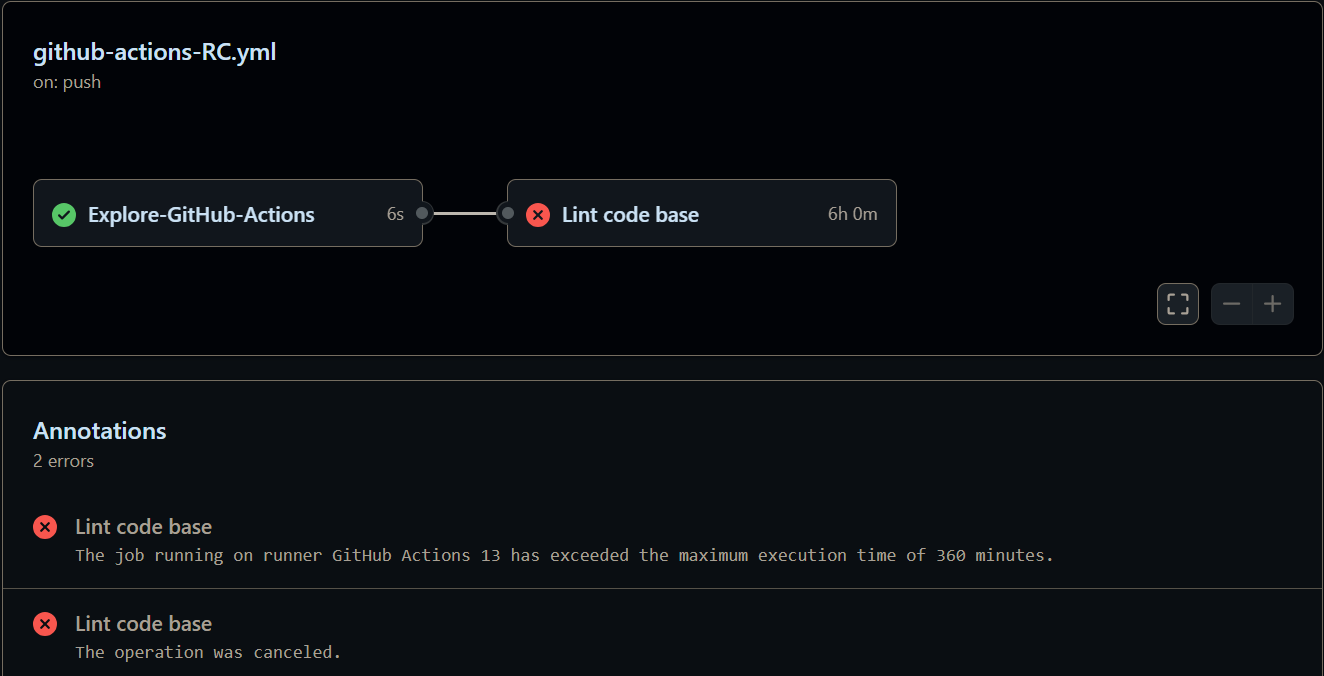
\includegraphics[width=0.7\textwidth]{lintCodebaseError.png}
  \caption{Lint codebase error}
  \label{FigUH}
\end{figure}

\newpage

\begin{landscape}
\section{Trace to Requirements}

See SRS Documentation at \href{https://github.com/Inreet-Kaur/capstone/blob/main/docs/SRS/SRS.pdf} {SRS document} for detailed Information.\\

\begin{table}[H]
  \centering
  \begin{tabular}{|c|c|c|c|c|c|c|c|c|c|c|c|c|c|}
  \hline
   Test ID & FR1 & FR2 & FR3 & FR4 & FR5 & FR6 & FR7 & FR8 & FR9 & FR10 & FR11 & FR12 & FR13 \\
  \hline
  test-FR1,4,8-1 & $\times$ & & & $\times$ & & & & $\times$ & & & & & \\
  \hline
  test-FR1,4,8-2 & $\times$ & & & $\times$ & & & & $\times$ & & & & & \\
  \hline
  test-FR2,5,9-1 & & $\times$ & & & $\times$ & & & & $\times$ & & & & \\
  \hline
  test-FR2,5,9-2 & & $\times$ & & & $\times$ & & & & $\times$ & & & & \\
  \hline
  test-FR3,6,10,11-1 & & & $\times$ & & & $\times$ & & & & $\times$ & $\times$ & & \\
  \hline
  test-FR3,6,10,11-2 & & & $\times$ & & & $\times$ & & & & $\times$ & $\times$ & & \\
  \hline
  test-FR7-1 & & & & & & & $\times$ & & & & & & \\
  \hline
  test-FR7-2 & & & & & & & $\times$ & & & & & & \\
  \hline
  test-FR11-1 & & & & & & & & & & & $\times$ & & \\
  \hline
  test-FR11-2 & & & & & & & & & & & $\times$ & & \\
  \hline
  test-FR12,13-1 & & & & & & & & & & & & $\times$ & $\times$ \\
  \hline
  test-FR12,13,IR5-1 & & & & & & & & & & & & $\times$ & $\times$ \\
  \hline
  test-FR12,13,IR5-2 & & & & & & & & & & & & $\times$ & $\times$ \\
  \hline
\end{tabular}
\caption{\bf Functional Requirements Tests Requirement Traceability} \label{tab:fr-test-traceability}
\end{table}

\end{landscape}
\newpage

\begin{table} [H]
  \centering
  \begin{tabular}{|c|c|c|c|c|c|c|c|c|c|}
    \hline
    TestID & NFR1 & NFR2 & NFR3 & NFR4 & NFR5 & NFR6 & NFR7 & NFR8 & NFR9 \\
    \hline
    test-AD1 & $\times$ & & & & & & & & \\
    \hline
    test-AD2 &  $\times$ & & & & & & & & \\
    \hline
    test-UR1 & & $\times$ &  & & & & & & \\
    \hline
    test-PR1 & & & $\times$ & & & & & & \\
    \hline
    test-OR1 & & & & $\times$ & & & & &  \\
    \hline
    test-MR1 & & & & & $\times$ & & & &\\
    \hline
    test-MR2 & & & & & $\times$ & & & &  \\
    \hline
    test-SR1 & & & & & & $\times$ & & &\\
    \hline
    test-CR1 & & & & & & & $\times$ & &\\
    \hline
    test-LR1 & & & & & & & & $\times$ &\\
    \hline
    test-LR2 & & & & & & & & $\times$ & \\
    \hline
    test-S1 & & & & & & & & & $\times$ \\
    \hline
  \end{tabular}
\caption{\bf Non-Functional Requirements Tests Requirement Traceability} \label{tab:nfr-test-traceability}
\end{table}

\begin{table} [H]
  \centering
  \begin{tabular}{|c|c|c|c|c|c|c|c|c|c|}
  \hline
  Test ID & AC1 & AC2 & IR1 & IR2 & IR3 & IR4 & IR5 & IR6 & IR7 \\
  \hline
  test-AC1-1 & $\times$ & & & & & & & & \\
  \hline
  test-AC1-2 & $\times$ & & & & & & & & \\
  \hline
  test-AC2-1 & & $\times$ & & & & & & & \\
  \hline
  test-IR1-1 & & & $\times$ & & & & & & \\
  \hline
  test-IR2-1  & & & & $\times$ & & & & &\\
  \hline
  test-IR3-1  & & & & & $\times$ & & & &\\
  \hline
  test-IR4-1  & & & & & & $\times$ & & & \\
  \hline
  test-FR12,13,IR5  & & & & & & & $\times$ & & \\
  \hline
  test-IR6-1  & & & & & & &  $\times$ & & \\
  \hline
  test-IR7-1  & & & & & & & &  $\times$ & \\
  \hline
\end{tabular}
\caption{\bf Safety and Security Requirements Tests Requirement Traceability} \label{tab:sns-test-traceability}
\end{table}

\newpage
		
\section{Trace to Modules}

See MG Documentation at \href{https://github.com/PKALXI/RapidCare/blob/main/docs/Design/SoftArchitecture/MG.pdf} {MG} for detailed Information.\\

\begin{table}[H]
  \centering
  \begin{tabular}{|c|c|c|c|c|c|c|c|c|c|c|c|c|c|}
  \hline
  Test ID & M1 & M2 & M3 & M4 & M5 & M6 & M7 & M8 & M9 & M10 & M11 & M12 \\
  \hline
  test-FR1,4,8-1 & & $\times$ & $\times$ & & & & & & & & $\times$ & $\times$ \\
  \hline
  test-FR1,4,8-2 & & $\times$ & $\times$ & & & & & & & & $\times$ & $\times$ \\
  \hline
  test-FR2,5,9-1 & & $\times$ & $\times$ & & & & & & & & $\times$ & $\times$ \\
  \hline
  test-FR2,5,9-2 & & $\times$ & $\times$ & & & & & & & & $\times$ & $\times$ \\
  \hline
  test-FR3,6,10,11-1 & & $\times$ & $\times$ & & & & & & & & $\times$ & $\times$ \\
  \hline
  test-FR3,6,10,11-2 & & $\times$ & $\times$ & & & & & & & & $\times$ & $\times$ \\
  \hline
  test-FR7-1 & $\times$ & $\times$ & $\times$ & & & $\times$ & & & & & & \\
  \hline
  test-FR7-2 & $\times$ & $\times$ & $\times$ & & & $\times$ & & & & & & \\
  \hline
  test-FR11-1 & & & $\times$ & & & $\times$ & $\times$ & $\times$ & & & & \\
  \hline
  test-FR11-2 & & & $\times$ & & & $\times$ & $\times$ & $\times$ & & & & \\
  \hline
  test-FR12,13-1 & & & $\times$ & & & $\times$ & & & $\times$ & $\times$ & & \\
  \hline
  test-FR12,13,IR5-1 & & & $\times$ & & & $\times$ & & & $\times$ & $\times$ & & \\
  \hline
  test-FR12,13,IR5-2 & & & $\times$ & & & $\times$ & & & $\times$ & $\times$ & & \\
  \hline
\end{tabular}
\caption{\bf Functional Requirements Tests Module Traceability} \label{tab:fr-test-traceability}
\end{table}

\begin{table} [H]
  \centering
  \begin{tabular}{|c|c|c|c|c|c|c|c|c|c|c|c|c|c|}
    \hline
    TestID & M1 & M2 & M3 & M4 & M5 & M6 & M7 & M8 & M9 & M10 & M11 & M12 \\
    \hline
    test-AD1 & & $\times$ & $\times$ & & & & & & & & &\\
    \hline
    test-AD2 & & $\times$ & $\times$ & & & & & & & & &\\
    \hline
    test-UR1 & $\times$ & $\times$ & $\times$ & $\times$ & $\times$ & $\times$ & $\times$ & $\times$ & $\times$ & $\times$ & $\times$ & $\times$ \\
    \hline
    test-PR1 & & & $\times$ & & & $\times$ & $\times$ & $\times$ & & & &\\
    \hline
    test-OR1 & $\times$ & $\times$ & $\times$ & $\times$ & $\times$ & $\times$ & $\times$ & $\times$ & $\times$ & $\times$ & $\times$ & $\times$ \\
    \hline
    test-MR1 & $\times$ & $\times$ & $\times$ & $\times$ & $\times$ & $\times$ & $\times$ & $\times$ & $\times$ & $\times$ & $\times$ & $\times$ \\
    \hline
    test-MR2 & $\times$ & $\times$ & $\times$ & $\times$ & $\times$ & $\times$ & $\times$ & $\times$ & $\times$ & $\times$ & $\times$ & $\times$ \\
    \hline
    test-SR1 & $\times$ & $\times$ & & & & $\times$ & & & & & & \\
    \hline
    test-CR1 & & $\times$ & $\times$ & & & & & & & & & \\
    \hline
    test-LR1 & & & & & & $\times$ & & & & & $\times$ & $\times$\\
    \hline
    test-LR2 & & & & & & $\times$ & & & & & $\times$ & $\times$\\
    \hline
    test-S1 & $\times$ & $\times$ & $\times$ & $\times$ & $\times$ & $\times$ & $\times$ & $\times$ & $\times$ & $\times$ & $\times$ & $\times$ \\
    \hline
  \end{tabular}
\caption{\bf Non-Functional Requirements Tests Module Traceability} \label{tab:nfr-test-traceability}
\end{table}

\begin{table} [H]
  \centering
  \begin{tabular}{|c|c|c|c|c|c|c|c|c|c|c|c|c|c|}
  \hline
  Test ID & M1 & M2 & M3 & M4 & M5 & M6 & M7 & M8 & M9 & M10 & M11 & M12 \\
  \hline
  test-AC1-1 & $\times$ & & & & & & & & & & & \\
  \hline
  test-AC1-2 & $\times$ & & & & & & & & & & & \\
  \hline
  test-AC2-1 & $\times$ & & & & & & & & & & & \\
  \hline
  test-IR1-1 & $\times$ & $\times$ & $\times$ & & & & & & & & $\times$ & $\times$\\
  \hline
  test-IR2-1 & & $\times$ & $\times$ & & & & & & & & $\times$ & $\times$\\
  \hline
  test-IR3-1 & & & & & & & & & $\times$ & $\times$ & &\\
  \hline
  test-IR4-1 & & $\times$ & $\times$ & & & & & & & & $\times$ & $\times$\\
  \hline
  test-IR6-1 & & & & & & & $\times$ & $\times$ & & & &\\
  \hline
  test-IR7-1 & & & & & & & $\times$ & $\times$ & & & &\\
  \hline
\end{tabular}
\caption{\bf Safety and Security Requirements Tests Module Traceability} \label{tab:sns-test-traceability}
\end{table}

\newpage

\section{Code Coverage Metrics}

The image below displays the code coverage matrix for UI, Patient Account Management, Administrator Account Management, and Authentication Modules. As can been in the figure below, the code coverage for all the files we created the unit tests for is 100\%. 

\begin{figure}[h]
  \centering
  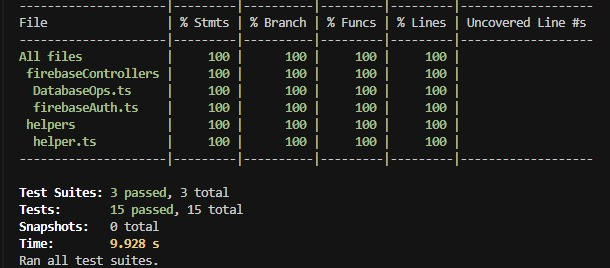
\includegraphics[width=0.7\textwidth]{CodeCoverageMetrics.jpg}
  \caption{Code Coverage Metrics}
  \label{FigUH}
\end{figure}

\bibliographystyle{plainnat}
\bibliography{../../refs/References}

\newpage{}
\section*{Appendix --- Reflection}

The information in this section will be used to evaluate the team members on the
graduate attribute of Reflection.

\input{../Reflection.tex}

\begin{enumerate}
  \item What went well while writing this deliverable?\\
  This document has let us strengthen the understanding about unit testing of all functional requirements as well as verification of all non-functional qualities of the system. While going through the outline of the document, we were able to conduct unit testing and compare it with the existing implementation. It also made us better execute the detailed procedure of system testing along with performing validation and verification of the system. 

  \item What pain points did you experience during this deliverable, and how did you resolve them?\\
  There are obstacles in any team project that must be overcome for it to proceed successfully. To ensure seamless operations, we had to develop a strategy for contributions. Since we already had the list of tests that were needed to be conducted for both functional and non-functional requirements, we divided them equally among all the team members. We also needed to create a schedule to contribute to the template and review each other's work in the best way possible. 

  \item Which parts of this document stemmed from speaking to your client(s) or a proxy (e.g. your peers)? Which ones were not, and why?\\
  The client's feedback helped us to understand the changes due to testing the requirements. Before Rev 0 demo, the team gave a demo to the supervisor about the system pretending the supervisor as the healthcare professional using the system. The supervisor then gave us some possible ways that the healthcare professional would like to use the system. This helped us to improve some features of the system such as whether prescription of a patient is being saved or not. If yes, then is it being stored within the system or on local machine. Furthermore, the section such as unit testing of all functional requirements stemmed from the collective ideas of our peers. We discussed different test cases that each requirement could possibly have along with how they will be implemented. In this way, we got diverse test cases and all team members were able to contribute especially in this critical section of the report.

  \item In what ways was the Verification and Validation (VnV) Plan different
  from the activities that were actually conducted for VnV?  If there were
  differences, what changes required the modification in the plan?  Why did
  these changes occur?  Would you be able to anticipate these changes in future
  projects?  If there weren't any differences, how was your team able to clearly
  predict a feasible amount of effort and the right tasks needed to build the
  evidence that demonstrates the required quality?  (It is expected that most
  teams will have had to deviate from their original VnV Plan.)\\
  VnV Plan was little bit different from the activities that were actually conducted and recorded in VnVReport. This is because VnV Plan includes one extra functional requirement test which needs to be deleted as the team has decided to not pursue with that functional requirement. Therefore, the team will modify the VnV Plan to remove that requirement. Additionally, as part of the modifications, the team removed some Non-Functional Requirements tests to reduce redundancy, such as test-S2, test-CR2, and test-PR1, and updated the traceability to the requirements for both Non-Functional Requirements tests and Safety and Security tests. These changes were made to streamline the testing process and ensure alignment with the system's goals. This change occurred as we went through every detail of our system and it turns out that functional requirement is not necessary for the system to accomplish its goal. Yes, we will be able to anticipate thus change in the future projects as going through every detail of the project review the necessary and non-necessary features of the product.  

\end{enumerate}

\end{document}